\section{Kasus Dasar}
\begin{longtable}{|c|>{\centering\arraybackslash}m{5.5cm}|>{\centering\arraybackslash}m{5.5cm}|}
    \caption{Hasil Pengujian pada Kasus Dasar} \label{tab:hasil_pengujian_1}                          \\

    \hline
    \textbf{No} & \textbf{Test Case}                                                 & \textbf{Hasil} \\
    \hline
    \endfirsthead

    \hline
    \textbf{No} & \textbf{Test Case}                                                 & \textbf{Hasil} \\
    \hline
    \endhead

    \hline
    \multicolumn{3}{r}{\textit{Lanjut ke halaman berikutnya}}                                         \\
    \hline
    \endfoot

    \hline
    \endlastfoot

    1           & 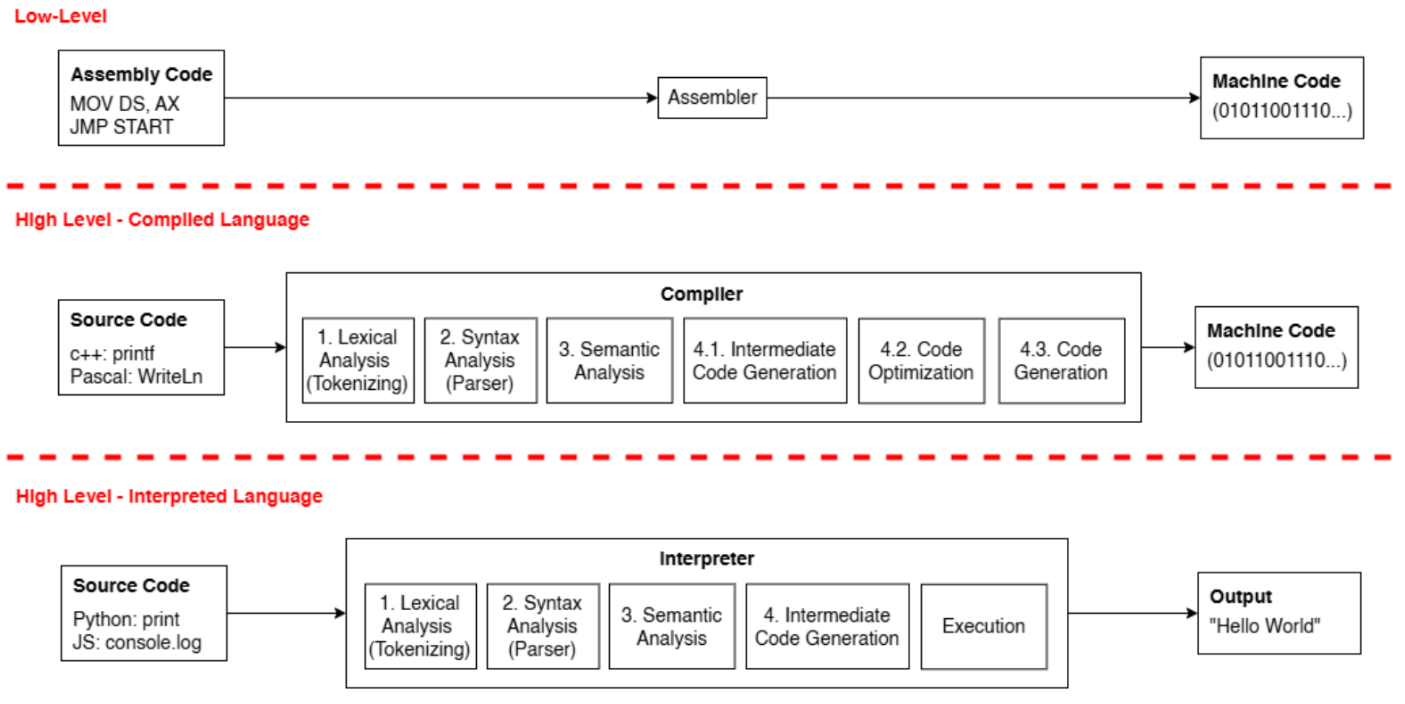
\includegraphics[width=5cm]{public/01-pendahuluan/tipe-bahasa.png}
                &
    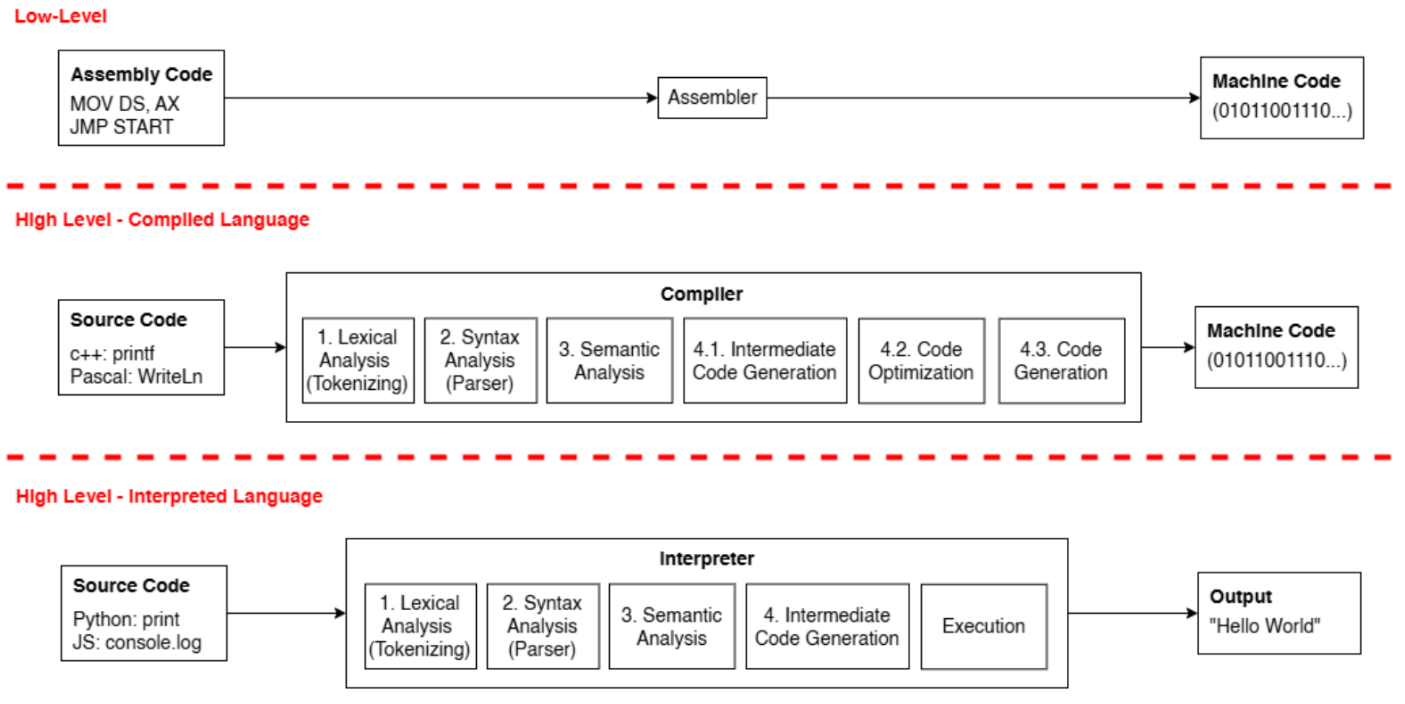
\includegraphics[width=5cm]{public/01-pendahuluan/tipe-bahasa.png}                                \\
    \hline

    2           &
    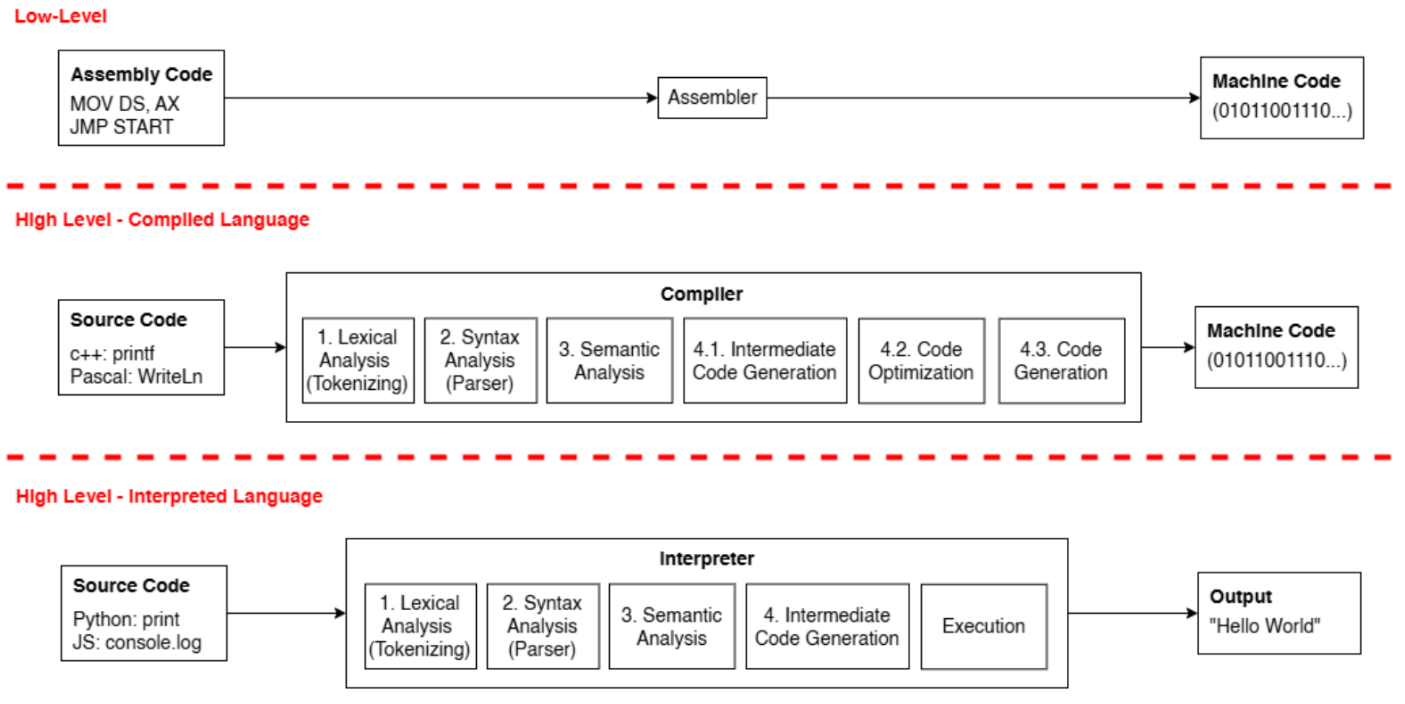
\includegraphics[width=5cm]{public/01-pendahuluan/tipe-bahasa.png}
                &
    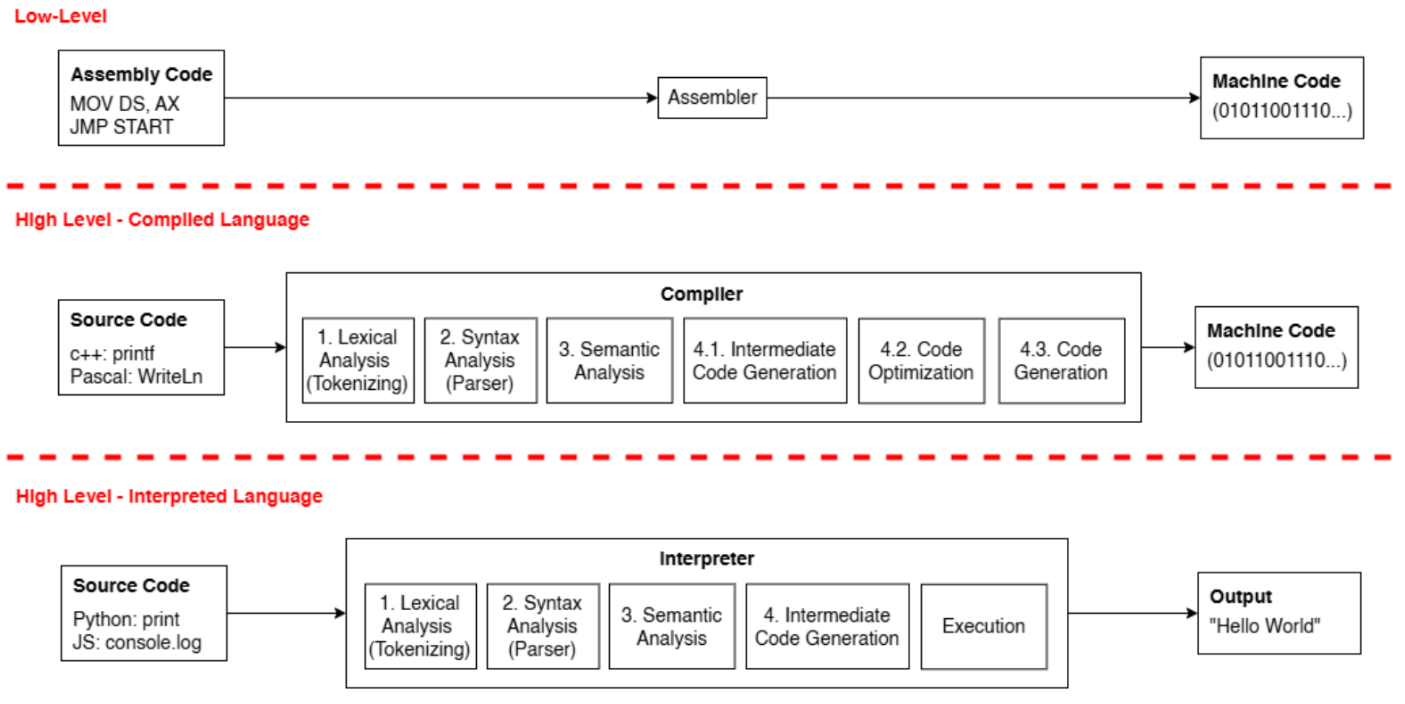
\includegraphics[width=5cm]{public/01-pendahuluan/tipe-bahasa.png}                                \\
    \hline

    3           &
    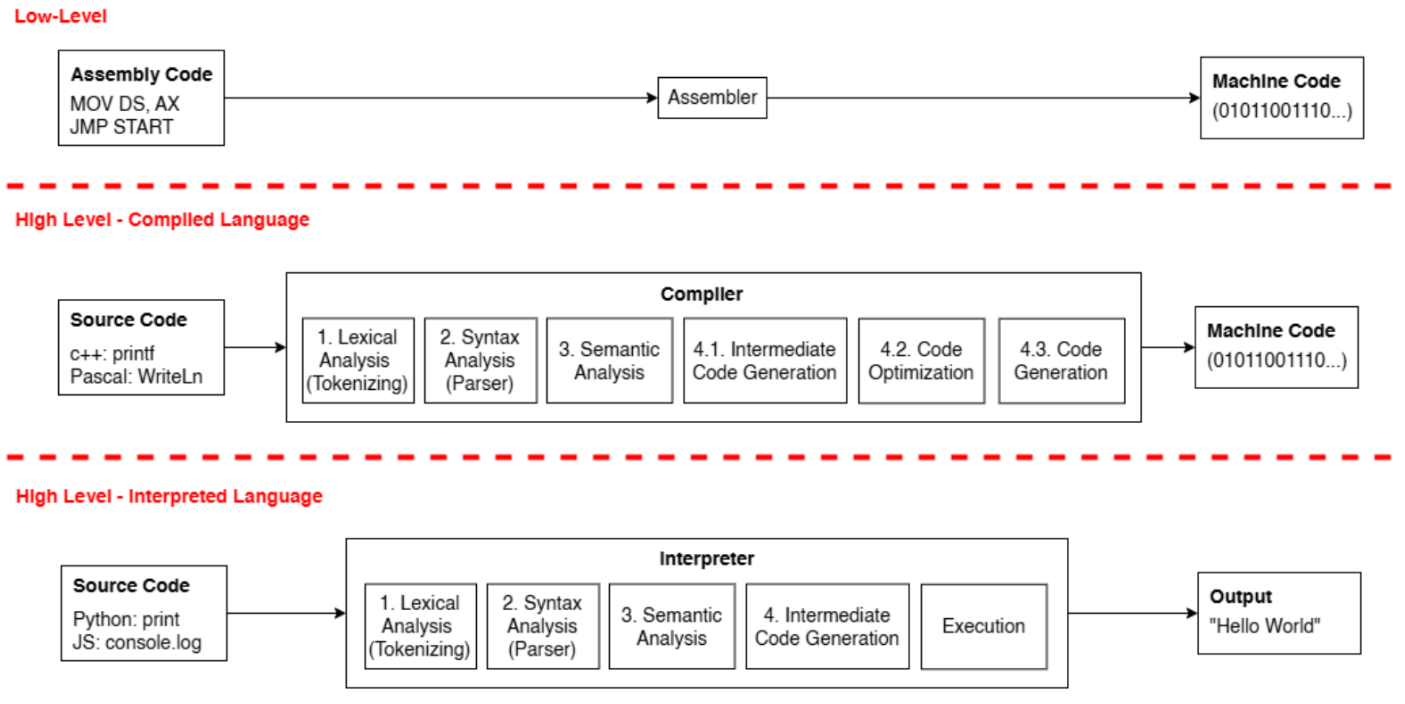
\includegraphics[width=5cm]{public/01-pendahuluan/tipe-bahasa.png}
                &
    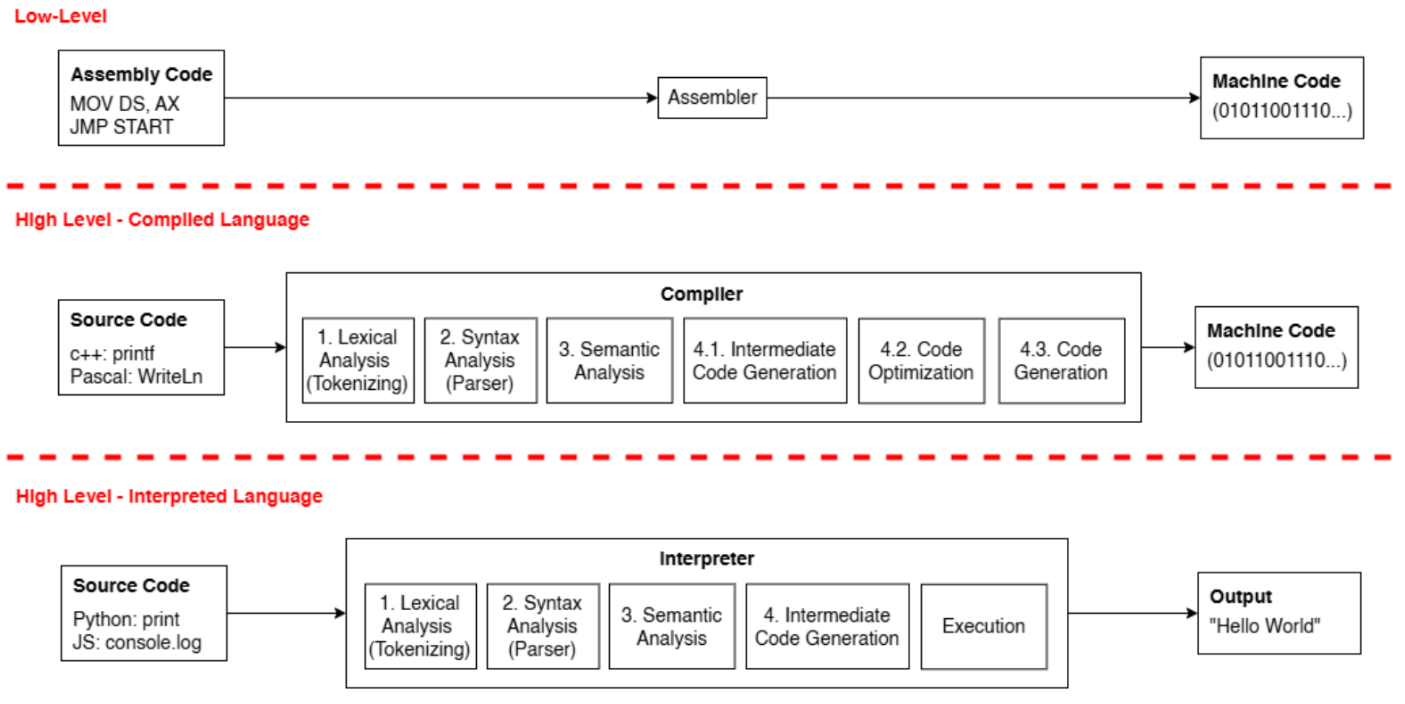
\includegraphics[width=5cm]{public/01-pendahuluan/tipe-bahasa.png}                                \\
    \hline

    4           &
    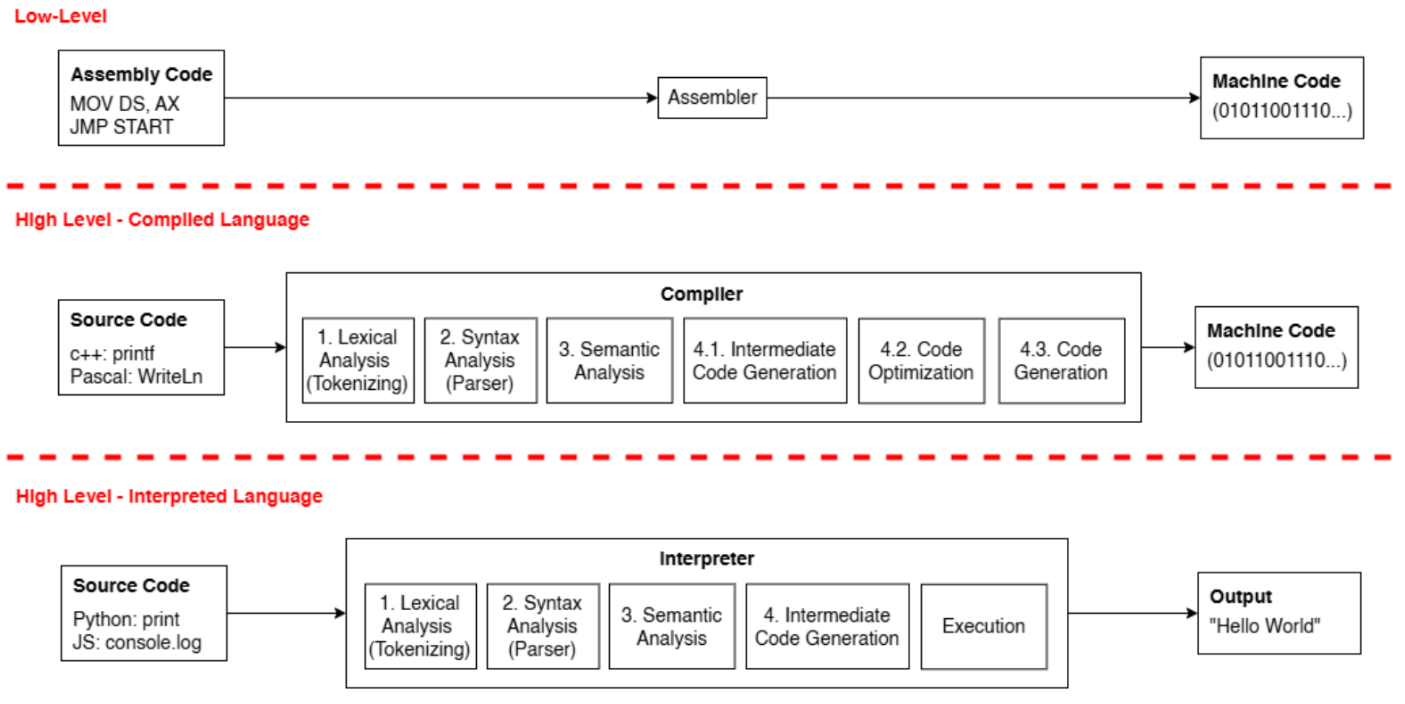
\includegraphics[width=5cm]{public/01-pendahuluan/tipe-bahasa.png}
                &
    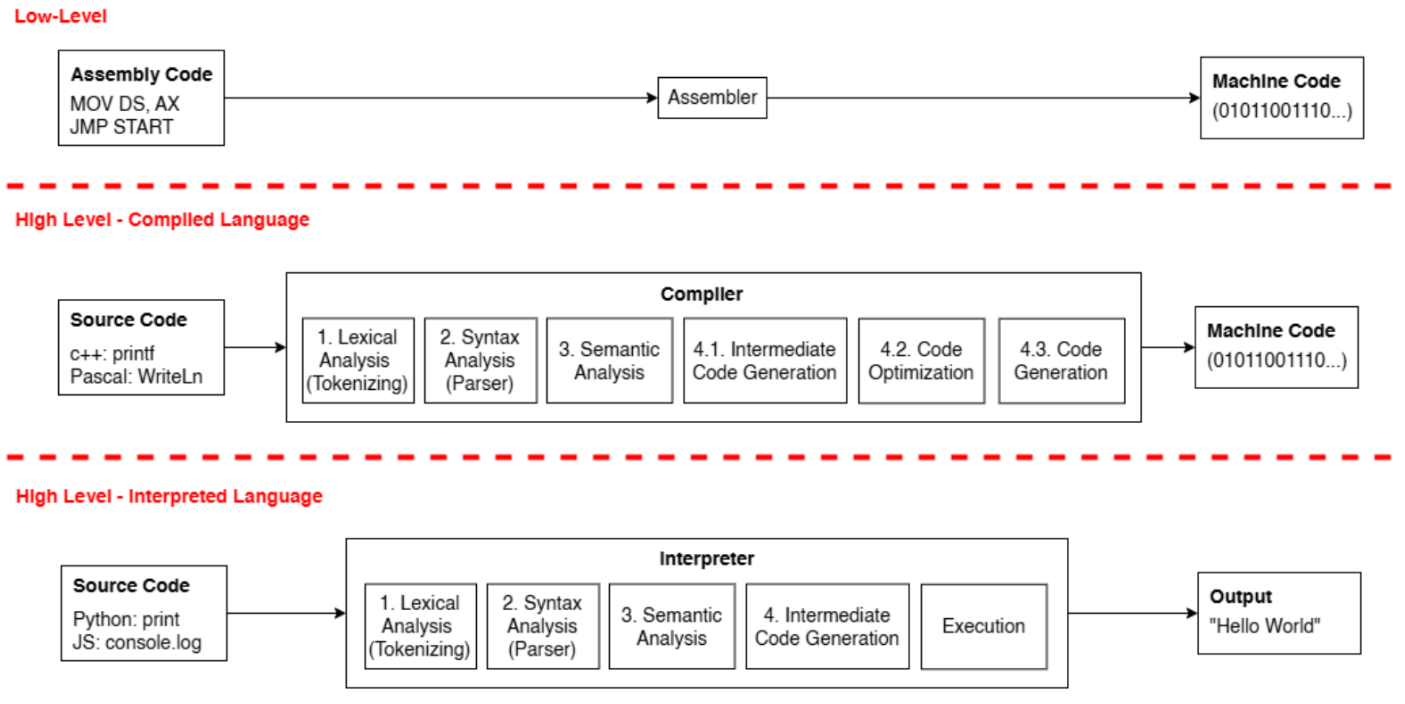
\includegraphics[width=5cm]{public/01-pendahuluan/tipe-bahasa.png}                                \\
    \hline


    % Tambahkan baris berikutnya di sini
\end{longtable}

\section{\textit{Edge Cases}}
\begin{longtable}{|c|>{\centering\arraybackslash}m{5.5cm}|>{\centering\arraybackslash}m{5.5cm}|}
    \caption{Hasil Pengujian pada Kasus Anomali} \label{tab:hasil_pengujian_2}                        \\

    \hline
    \textbf{No} & \textbf{Test Case}                                                 & \textbf{Hasil} \\
    \hline
    \endfirsthead

    \hline
    \textbf{No} & \textbf{Test Case}                                                 & \textbf{Hasil} \\
    \hline
    \endhead

    \hline
    \multicolumn{3}{r}{\textit{Lanjut ke halaman berikutnya}}                                         \\
    \hline
    \endfoot

    \hline
    \endlastfoot

    1           & 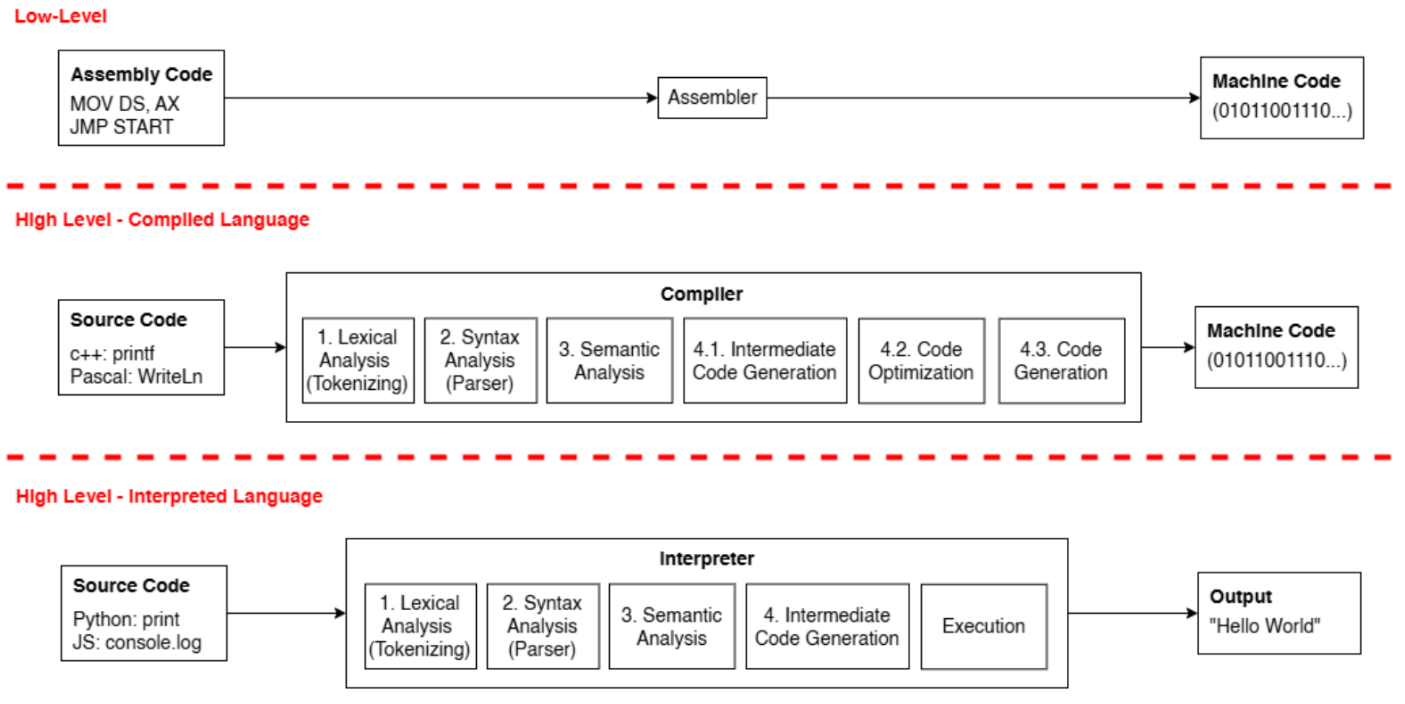
\includegraphics[width=5cm]{public/01-pendahuluan/tipe-bahasa.png}
                &
    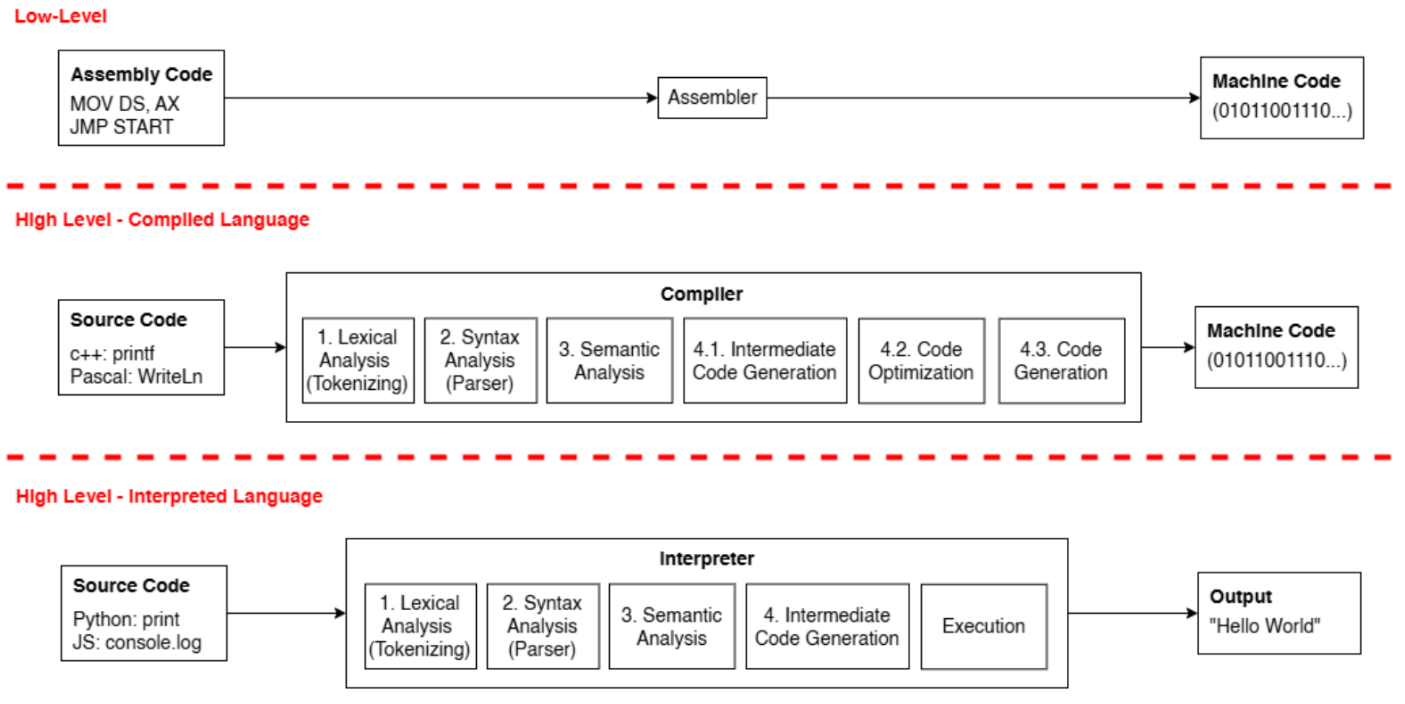
\includegraphics[width=5cm]{public/01-pendahuluan/tipe-bahasa.png}                                \\
    \hline

    2           &
    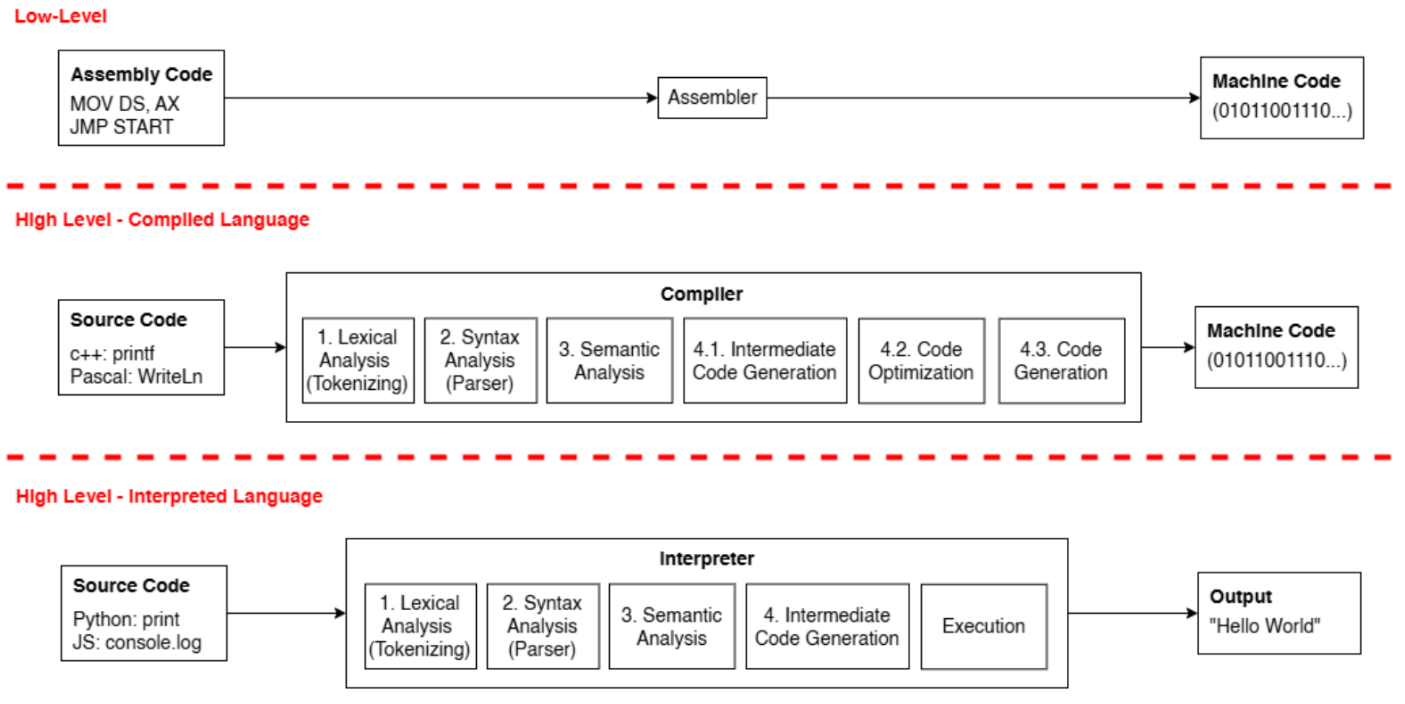
\includegraphics[width=5cm]{public/01-pendahuluan/tipe-bahasa.png}
                &
    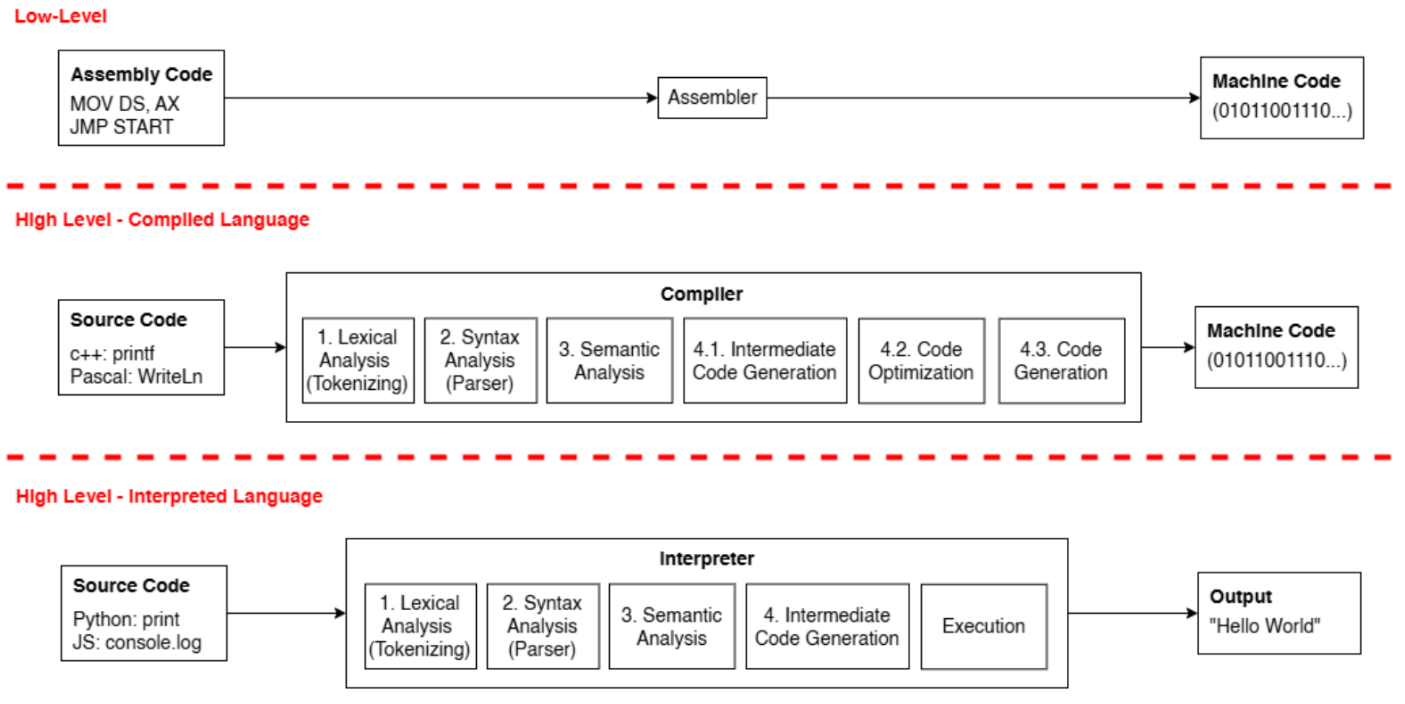
\includegraphics[width=5cm]{public/01-pendahuluan/tipe-bahasa.png}                                \\
    \hline

    3           &
    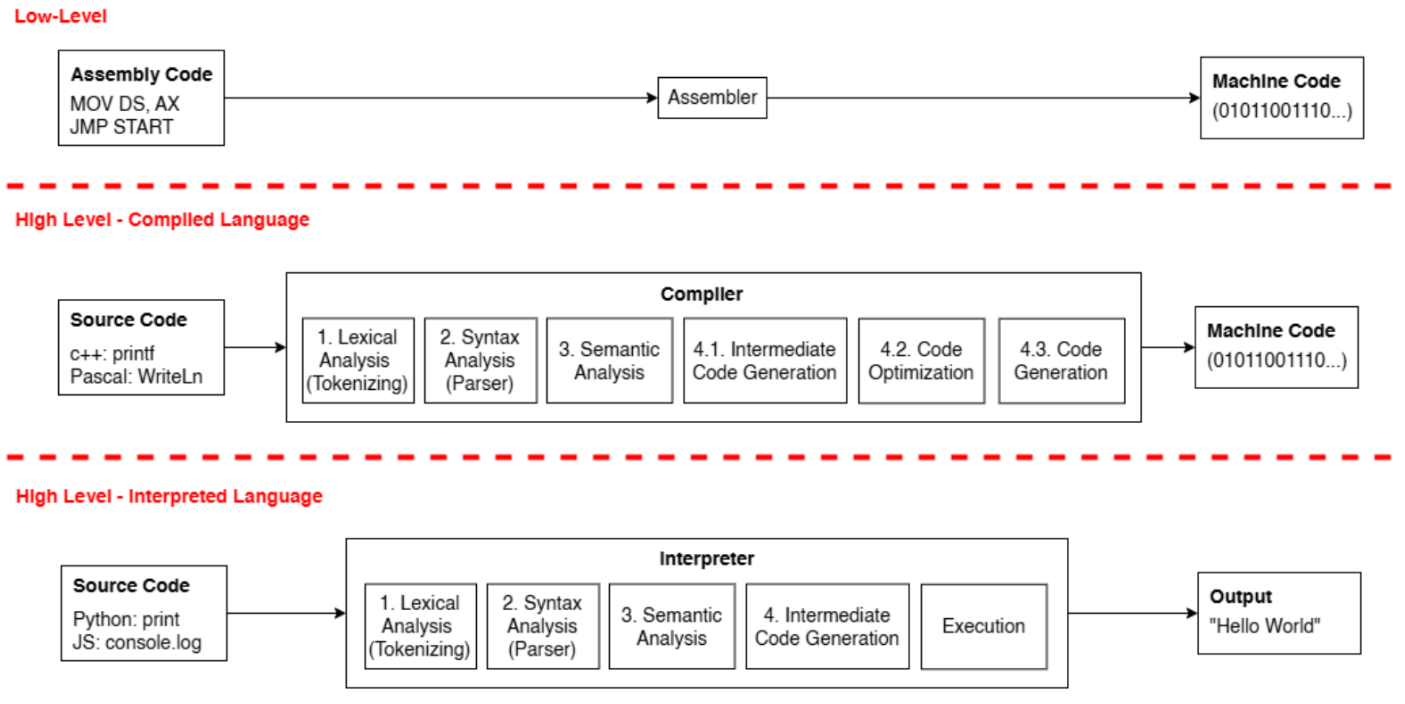
\includegraphics[width=5cm]{public/01-pendahuluan/tipe-bahasa.png}
                &
    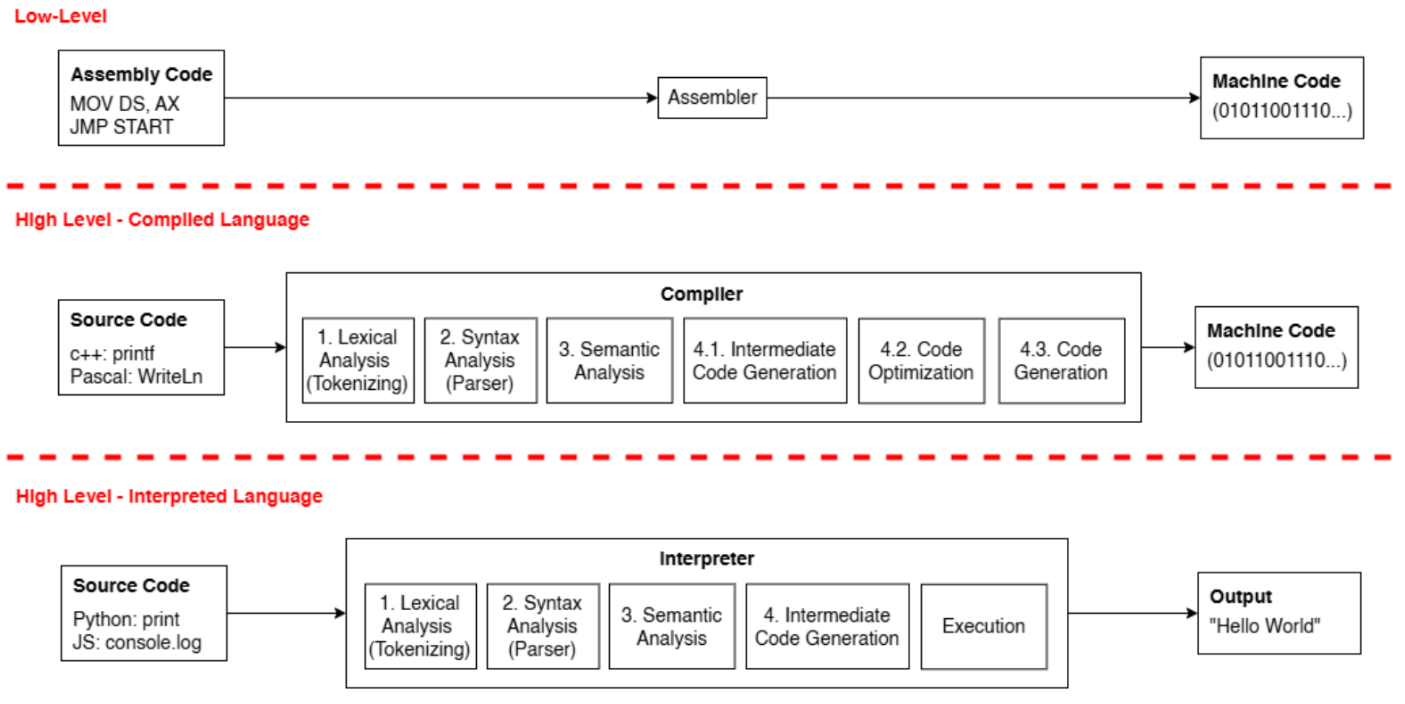
\includegraphics[width=5cm]{public/01-pendahuluan/tipe-bahasa.png}                                \\
    \hline

    4           &
    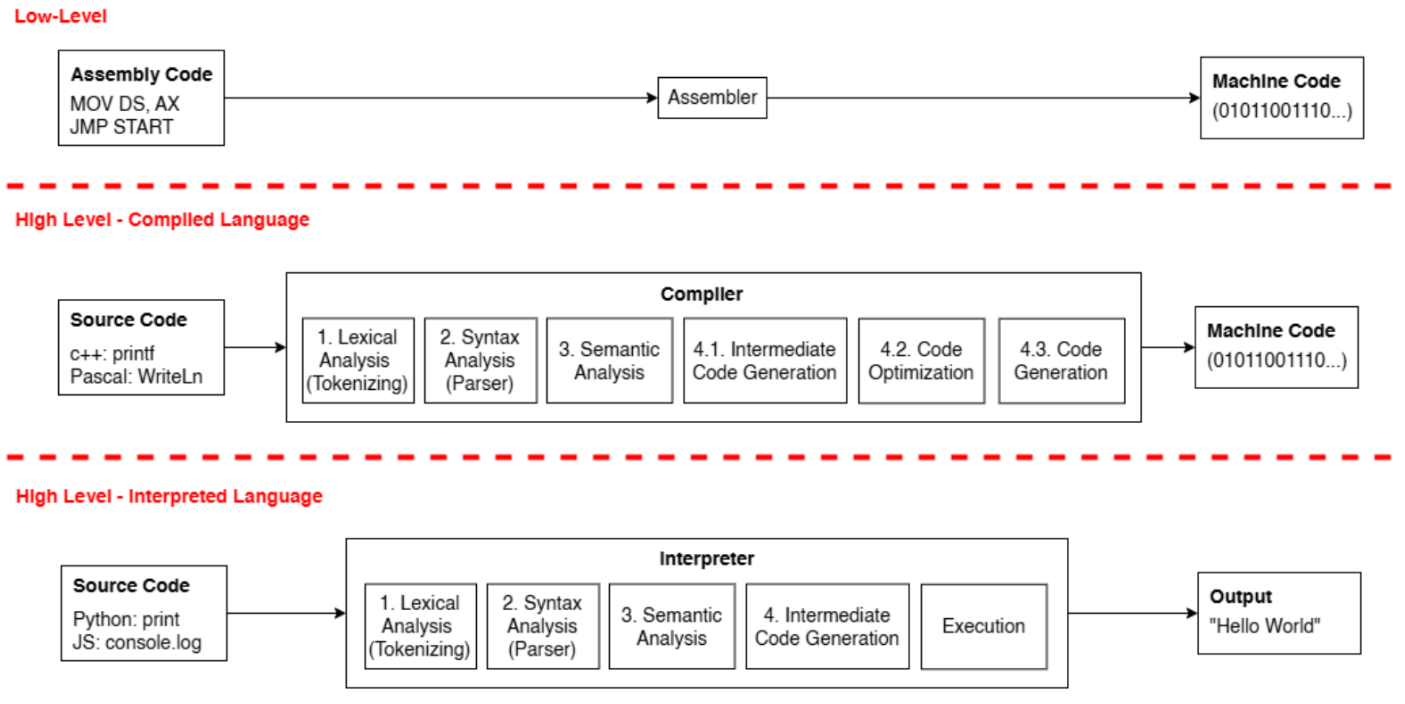
\includegraphics[width=5cm]{public/01-pendahuluan/tipe-bahasa.png}
                &
    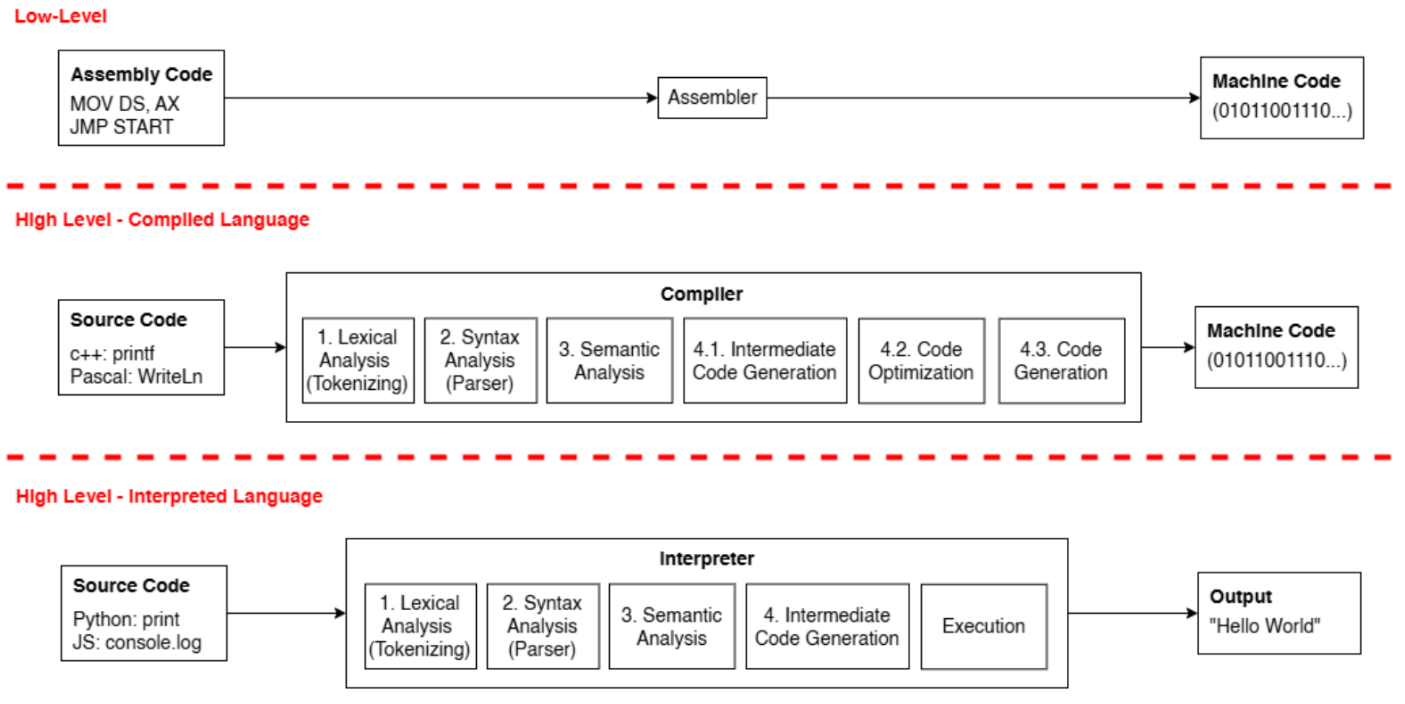
\includegraphics[width=5cm]{public/01-pendahuluan/tipe-bahasa.png}                                \\
    \hline


    % Tambahkan baris berikutnya di sini
\end{longtable}